\documentclass[a4paper,12pt]{article}
\usepackage{../packages/coursCollege}
\newcommand{\Chapitre}{Analyse combinatoire}
\renewcommand{\path}{../../}

\usepackage[    %backend=biber, 
    natbib=true,
    style=numeric,
    sorting=none]{biblatex}  % Load biblatex for bibliography handling
\addbibresource{biblio-der.bib}  
\renewcommand\refname{Sources}
\renewcommand{\cours}{3MA2~--~EG~--~ns~--~2025-2026}
\usepackage[edges]{forest}

% Define styles for the nodes
\forestset{
  decision/.style={
    draw,
    rounded corners,
    fill=LightSteelBlue!30,
    align=center,
    minimum height=1.5cm,
    text width=3.5cm,
    font=\small,
  },
  formula/.style={
    draw,
    fill=LightGrey!20,
    align=center,
    font=\small,
  },
  root/.style={
    decision,
    fill=IndianRed!40,
    font=\small\bfseries,
  }
}

\begin{document}

\section*{Résumé}

\begin{center}
\begin{forest}
  for tree={
    grow=south,            % Tree grows downwards
    parent anchor=south,   % Edges start from the bottom of parent nodes
    child anchor=north,    % Edges end at the top of child nodes
    l sep=1.5cm,           % Vertical distance between levels
    s sep=0.2cm,           % Horizontal distance between siblings
    forked edges,          % Edges fork from the parent node
    edge={draw, -latex'},  % Style for the arrows
  }
[Problème de\\dénombrement, root
  [L'ordre compte-t-il ?, decision
    [{$n=k$ ? \\ (Tous les éléments\\ sont-ils utilisés ?)}, decision, edge label={node[midway,left,font=\footnotesize]{oui}}
      [{Y a-t-il des éléments \\ identiques ?}, decision, edge label={node[midway,left,font=\footnotesize]{oui}}
        [Permutations avec répétitions \\ {$\overline{P}(n_1, n_2, \dots) = \dfrac{n!}{n_1!n_2!\cdots}$}, formula, edge label={node[midway,left,font=\footnotesize]{oui}}]
        [Permutations simples \\ $P_n = n!$, formula, edge label={node[midway,right,font=\footnotesize]{non}}]
      ]
      [{Répétitions possibles ?}, decision, edge label={node[midway,right,font=\footnotesize]{non}}
        [Arrangements avec répétition \\ $\overline{A_k^n} = n^k$, formula, edge label={node[midway,right,font=\footnotesize]{oui}}]
        [Arrangements simples \\ $A_k^n = \dfrac{n!}{(n-k)!}$, formula, edge label={node[midway,left,font=\footnotesize]{non}}]
      ]
    ]
    [{Répétitions possibles ?}, decision, edge label={node[midway,right,font=\footnotesize]{non}}
      [Combinaisons avec répétition \\ $\overline{C_k^n} = \dbinom{n+k-1}{k} = \dfrac{(n+k-1)!}{k!(n-1)!}$, formula, edge label={node[midway,right,font=\footnotesize]{oui}}]
      [Combinaisons simples \\ $C_k^n = \dbinom{n}{k} = \dfrac{n!}{k!(n-k)!}$, formula, edge label={node[midway,left,font=\footnotesize]{non}}]
    ]
  ]
]
\end{forest}
\end{center}
\tocloftpagestyle{fancy}
% Reduce space between section entries
\setlength{\cftbeforesecskip}{2pt}

% Reduce indentation for section entries
\setlength{\cftsecindent}{1em}

\begin{center}
	{\bfseries \Huge Chapitre 1~: \\Analyse combinatoire}
	

	\vspace{1cm}
\begin{tikzpicture}[scale=2]
  % Draw a simple tree structure representing combinatorial analysis
  \node[circle, draw, minimum size=1cm] at (0,0) {n};
  \draw[thick] (0,0) -- (-1,-1);
  \draw[thick] (0,0) -- (0,-1);
  \draw[thick] (0,0) -- (1,-1);
  \node[circle, draw, minimum size=0.8cm] at (-1,-1) {$k_1$};
  \node[circle, draw, minimum size=0.8cm] at (0,-1) {$k_2$};
  \node[circle, draw, minimum size=0.8cm] at (1,-1) {$k_3$};
  
  % Add some combinatorial symbols
  \node at (-2,0.5) {$C_k^n$};
  \node at (2,0.5) {$A_k^n$};
  \node at (0,1.5) {$P_n = n!$};
\end{tikzpicture}
\end{center}
\vspace{-1cm}
\tableofcontents
\newpage

\section*{Prérequis}
Avant de commencer ce chapitre, je m'assure d'être capable de 
\bigskip

\begin{tblr}{
  colspec = {|l|X[2]|c|c|},     % Adjusted column widths
  row{1} = {bg=gray!20, font=\bfseries}, % Header styling
  rows = {valign=m, ht=2cm},    % Minimum row height for QR codes
  vlines,
  hlines,
  width = \textwidth,           % Table spans full text width
}
%------------ Header -------------------------------------------------
Catégorie & 
Compétence & 
QR Code & 
Validation \\
%------------ Calcul numérique ---------------------------------------
\SetCell[r=2]{l, bg=blue!10} {\textbf{Calcul\\numérique}} &
Effectuer des calculs avec des puissances &
\qrcode[height=2.5cm]{https://example.com/puissances} &
\checkBox \\
&
Calculer avec des fractions &
\qrcode[height=2.5cm]{https://example.com/fractions} &
\checkBox \\
%------------ Algèbre ------------------------------------------------
\SetCell[r=2]{l, bg=green!10} {\textbf{Algèbre}} &
Résoudre des équations simples &
\qrcode[height=2.5cm]{https://example.com/equations} &
\checkBox \\
&
Simplifier des expressions algébriques &
\qrcode[height=2.5cm]{https://example.com/simplification} &
\checkBox \\
%------------ Logique ------------------------------------------------
\SetCell[r=1]{l, bg=orange!10} {\textbf{Logique}} &
Comprendre le principe de récurrence &
\qrcode[height=2.5cm]{https://example.com/recurrence} &
\checkBox \\
\end{tblr}

\vspace{1em}

\textit{Note: Scannez les codes QR pour accéder aux ressources d'apprentissage correspondantes.}

\newpage

\section{Outils de dénombrement}

\subsection{Exemples introductifs}

\begin{exemple}
	\tcblower
	{\bfseries Le problème de bébé Luca} -- 
	Bébé Luca adore déplacer les lettres aimantées qui se trouvent sur le frigo. S'il joue avec le A, le D et le F, combien de «mots» peut-il former ? (On ne cherche pas que le mot ait du sens en français).

	\begin{tasks}(1)
		\task Dresser la liste de tous les mots possibles.
		
		ADF, AFD, DAF, DFA, FAD, FDA

		\task Compléter l'arbre en indiquant clairement les légendes sur les branches et au bout des chemins.

		\begin{center}
		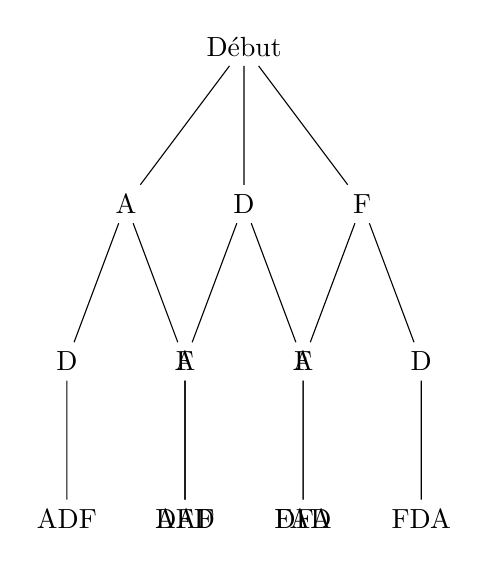
\begin{tikzpicture}[level distance=2cm, sibling distance=1.5cm]
		\node {Début}
		  child {node {A}
		    child {node {D}
		      child {node {ADF}}
		    }
		    child {node {F}
		      child {node {AFD}}
		    }
		  }
		  child {node {D}
		    child {node {A}
		      child {node {DAF}}
		    }
		    child {node {F}
		      child {node {DFA}}
		    }
		  }
		  child {node {F}
		    child {node {A}
		      child {node {FAD}}
		    }
		    child {node {D}
		      child {node {FDA}}
		    }
		  };
		\end{tikzpicture}
		\end{center}
	\end{tasks}
\end{exemple}

\begin{definition}
	Arbre de dénombrement
	\tcblower
	Un \emph{arbre} est un schéma permettant de décrire et de dénombrer tous les résultats possibles d'une suite finie d'opérations. Dans ce cas, on commence par tracer les branches représentant les différents choix pour « la première étape », puis au bout de chaque branche on trace les différents choix pour « la deuxième étape », etc. Le nombre de possibilités s'obtient en comptant le nombre de chemins possibles (en allant du début de l'arbre jusqu'au bout de la dernière feuille).
\end{definition}

\begin{exemplesuite}
	\tcblower
	\begin{tasks}(1)
		\task Compter le nombre de mots possibles en multipliant le nombre de possibilités pour chaque étape.

		\begin{center}
		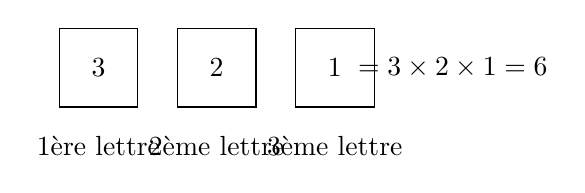
\begin{tikzpicture}
		\draw (0,0) rectangle (1,1);
		\draw (1.5,0) rectangle (2.5,1);
		\draw (3,0) rectangle (4,1);
		\node at (0.5,0.5) {3};
		\node at (2,0.5) {2};
		\node at (3.5,0.5) {1};
		\node at (0.5,-0.5) {1ère lettre};
		\node at (2,-0.5) {2ème lettre};
		\node at (3.5,-0.5) {3ème lettre};
		\node at (5,0.5) {$= 3 \times 2 \times 1 = 6$};
		\end{tikzpicture}
		\end{center}

		\task S'il a maintenant 10 lettres différentes à disposition et qu'il décide d'« écrire » un mot de 3 lettres, combien pourra-t-il former de mots différents ?

		\begin{center}
		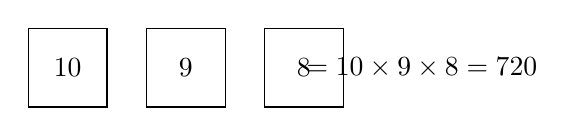
\begin{tikzpicture}
		\draw (0,0) rectangle (1,1);
		\draw (1.5,0) rectangle (2.5,1);
		\draw (3,0) rectangle (4,1);
		\node at (0.5,0.5) {10};
		\node at (2,0.5) {9};
		\node at (3.5,0.5) {8};
		\node at (5,0.5) {$= 10 \times 9 \times 8 = 720$};
		\end{tikzpicture}
		\end{center}

		\task S'il a maintenant toutes les lettres de l'alphabet à disposition et qu'il décide d'« écrire » cette fois-ci un mot de 5 lettres, combien pourra-t-il former de mots différents ?

		Il y a 5 étapes, donc 5 carrés :

		\begin{center}
		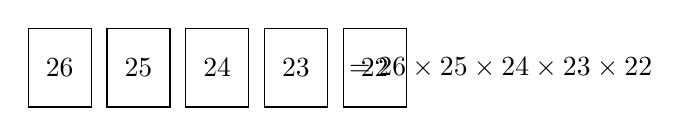
\begin{tikzpicture}
		\draw (0,0) rectangle (0.8,1);
		\draw (1,0) rectangle (1.8,1);
		\draw (2,0) rectangle (2.8,1);
		\draw (3,0) rectangle (3.8,1);
		\draw (4,0) rectangle (4.8,1);
		\node at (0.4,0.5) {26};
		\node at (1.4,0.5) {25};
		\node at (2.4,0.5) {24};
		\node at (3.4,0.5) {23};
		\node at (4.4,0.5) {22};
		\node at (6,0.5) {$= 26 \times 25 \times 24 \times 23 \times 22$};
		\end{tikzpicture}
		\end{center}
	\end{tasks}
\end{exemplesuite}

\begin{thm}
	Principe de décomposition
	\tcblower
	Si une expérience peut se décomposer en $k$ phases successives, ces dernières pouvant s'effectuer respectivement de $n_1, n_2, \ldots, n_k$ manières, alors l'expérience peut se réaliser de $n_1 \cdot n_2 \cdot \ldots \cdot n_k$ manières différentes.
\end{thm}

\section{Factorielles}

\begin{definition}
	Factorielle
	\tcblower
	Soit $n$ un entier positif ou nul. On appelle \emph{$n$ factorielle}, noté $n!$, le produit des nombres entiers de 1 à $n$.
	\[n! = \begin{cases}
	1 & \text{si } n = 0 \\
	1 \cdot 2 \cdot 3 \cdot \ldots \cdot n & \text{si } n > 0
	\end{cases}\]
\end{definition}

\begin{remarque}
	\tcblower
	Sur la calculatrice, appuyer sur la touche $prb$ puis sélectionner $!$.
\end{remarque}

\begin{exemple}
	\tcblower
	\begin{tasks}(4)
		\task $0! = 1$
		\task $5! = 1 \cdot 2 \cdot 3 \cdot 4 \cdot 5 = 120$
		\task $69! = 1{,}711 \times 10^{98}$
		\task $70! = 1{,}198 \times 10^{100}$
	\end{tasks}
\end{exemple}

\section{Permutations}

\subsection{Permutations simples}

\begin{definition}
	Permutation simple
	\tcblower
	Si on classe dans un ordre particulier $n$ objets distincts, on forme une \emph{permutation simple}. Le nombre $P_n$ de permutations simples est
	\[P_n = n!\]
\end{definition}

\begin{exemple}
	\tcblower
	Combien d'anagrammes du mot LAIT (même sans signification en français) peut-on former ?

	Le mot LAIT contient 4 lettres distinctes. Le nombre d'anagrammes est donc :
	\[P_4 = 4! = 24\]
\end{exemple}

\subsection{Permutations avec répétition}

\begin{exemple}
	\tcblower
	{\bfseries Illustration} -- Combien de mots distincts peut-on écrire avec les 5 lettres du mot ERRER ?

	Pour répondre à cette question, on va considérer les permutations simples des 5 objets distincts $e_1, r_1, r_2, e_2, r_3$. On trouve $5! = 120$ permutations.

	Parmi celles-ci, certaines sont indiscernables si on utilise le même graphisme pour toutes les lettres.

	\begin{itemize}
		\item En partant du « mot » ERRER, en permutant les trois $r$ on trouve $3! = 6$ fois le mot ERRER :
		\begin{center}
		$e_1r_1r_2e_2r_3$, $e_1r_2r_1e_2r_3$, $e_1r_3r_1e_2r_2$, $e_1r_1r_3e_2r_2$, $e_1r_2r_3e_2r_1$, $e_1r_3r_2e_2r_1$
		\end{center}
		
		\item Puis, en permutant les deux $e$, on multiplie encore toutes ces possibilités par $2! = 2$.
	\end{itemize}

	En conclusion, chacune des 120 permutations simples des objets $e_1, r_1, r_2, e_2, r_3$ contient $3! \times 2! = 12$ répétitions.

	Pour répondre à la question, on doit donc calculer :
	\[\frac{5!}{3! \times 2!} = \frac{120}{6 \times 2} = \frac{120}{12} = 10\]

	Il s'agit des « mots » : RRREE, RRERE, RREER, RERRE, RERER, REERR, ERRRE, ERRER, ERERR, EERRR.
\end{exemple}

\begin{definition}
	Permutation avec répétitions
	\tcblower
	Si on classe dans un ordre particulier $n$ éléments dont $n_1$ sont identiques de type 1, $n_2$ identiques de type 2, \ldots, $n_p$ identiques de type $p$, alors on forme une \emph{permutation avec répétitions}. Le nombre $\overline{P}(n_1, n_2, \ldots, n_p)$ de permutations avec répétitions est
	\[\overline{P}(n_1, n_2, \ldots, n_p) = \frac{n!}{n_1! \cdot n_2! \cdot \ldots \cdot n_p!}\]
	avec $n = n_1 + n_2 + \cdots + n_p$.
\end{definition}

\begin{exemple}
	\tcblower
	On compose des signaux en alignant 12 drapeaux : 4 blancs, 3 bleus, 3 rouges et 2 verts. Combien de signaux peut-on former ?

	On a $n = 12$ drapeaux au total avec :
	\begin{itemize}
		\item $n_1 = 4$ drapeaux blancs
		\item $n_2 = 3$ drapeaux bleus  
		\item $n_3 = 3$ drapeaux rouges
		\item $n_4 = 2$ drapeaux verts
	\end{itemize}

	Le nombre de signaux possibles est :
	\[\overline{P}(4,3,3,2) = \frac{12!}{4! \cdot 3! \cdot 3! \cdot 2!} = \frac{479~001~600}{24 \cdot 6 \cdot 6 \cdot 2} = \frac{479~001~600}{1~728} = 277~200\]
\end{exemple}

\section{Arrangements}

\subsection{Arrangements simples}

\begin{definition}
	Arrangement simple
	\tcblower
	Si, parmi $n$ éléments distincts, on choisit $k$ éléments distincts en les classant dans un ordre particulier, on forme un \emph{arrangement simple} de $k$ éléments choisis parmi $n$. Le nombre $A_k^n$ d'arrangements simples est
	\[A_k^n = n(n-1)(n-2)\ldots(n-k+1) = \frac{n!}{(n-k)!}\]
	avec $k \leq n$.
\end{definition}

\begin{remarque}
	\tcblower
	Sur la calculatrice, appuyer sur la touche $nPr$.
\end{remarque}

\begin{exemple}
	\tcblower
	Une course de chevaux compte 15 partants. Combien y a-t-il de possibilités de jouer un quarté (i.e. pronostiquer l'ordre d'arrivée des 4 premiers de la course) ?

	Il s'agit d'un arrangement de 4 éléments choisis parmi 15 :
	\[A_4^{15} = \frac{15!}{(15-4)!} = \frac{15!}{11!} = 15 \times 14 \times 13 \times 12 = 32~760\]
\end{exemple}

\begin{remarque}
	\tcblower
	\begin{enumerate}
		\item Une permutation simple est un cas particulier d'arrangement simple où on choisit $n$ éléments parmi $n$.
		\item Dans un arrangement simple, $k > n$ n'est pas possible, car on ne peut pas choisir plus d'éléments que ce qu'on a à disposition sans les répéter.
	\end{enumerate}
\end{remarque}

\subsection{Arrangements avec répétitions}

\begin{definition}
	Arrangement avec répétitions
	\tcblower
	Si, parmi $n$ éléments distincts, on choisit $k$ éléments distincts ou non (répétitions possibles) en les classant dans un ordre particulier, on forme un \emph{arrangement avec répétitions} de $k$ éléments choisis parmi $n$. Le nombre $\overline{A_k^n}$ d'arrangements avec répétitions est
	\[\overline{A_k^n} = n^k\]
\end{definition}

\begin{exemple}
	\tcblower
	\begin{tasks}(1)
		\task {\bfseries Exemple 1} -- Les plaques d'immatriculation d'un pays sont formées d'exactement quatre lettres de l'alphabet latin. Combien de voitures peut-on immatriculer dans ce pays ?

		Il y a 26 lettres dans l'alphabet latin et on forme des mots de 4 lettres avec répétitions possibles :
		\[\overline{A_4^{26}} = 26^4 = 456~976\]

		\task {\bfseries Exemple 2} -- On dispose des trois premières lettres de l'alphabet (A, B et C). Combien de mots de 5 lettres peut-on former avec ces 3 lettres ?

		\[\overline{A_5^3} = 3^5 = 243\]
	\end{tasks}
\end{exemple}

\section{Combinaisons}

\subsection{Illustration}

\begin{exemple}
	\tcblower
	Pour un mini tournoi de basket, combien d'équipes de 3 personnes peut-on former à partir d'une classe de 21 élèves ?

	\begin{tasks}(1)
		\task Si on utilise la formule des arrangements simples, combien compte-t-on de possibilités pour choisir ces 3 personnes ?
		
		\[A_3^{21} = \frac{21!}{18!} = 21 \times 20 \times 19 = 7~980\]

		\task Mais en réalité, on a compté plusieurs fois la même équipe. Donner un exemple avec les personnes de la classe :
		
		On a compté l'équipe avec Alice, Bob, Charlie qui est la même équipe que Bob, Alice, Charlie ou Charlie, Bob, Alice, etc.

		\task Il faudra donc diviser le nombre trouvé en a) par le nombre de possibilités de déplacer trois personnes, autrement dit par une permutation de 3.
		
		Ce qui donne $\frac{7~980}{3!} = \frac{7~980}{6} = 1~330$.

		\task D'une façon générale, nous avons fait :
		\[\frac{A_3^{21}}{P_3} = \frac{A_3^{21}}{3!}\]
	\end{tasks}
\end{exemple}

\subsection{Définition}

\begin{definition}
	Combinaison
	\tcblower
	Si, parmi $n$ éléments distincts, on choisit $k$ éléments distincts sans tenir compte de l'ordre, on forme une \emph{combinaison} de $k$ éléments choisis parmi $n$. Le nombre $C_k^n$ de combinaisons simples est
	\[C_k^n = \frac{n!}{(n-k)! \cdot k!}\]
	avec $k \leq n$.
\end{definition}

\begin{remarque}
	\tcblower
	Sur la calculatrice, appuyer sur la touche $prb$ puis sélectionner la 2ème ligne où est affiché $nCr$ avec $r = k$.
\end{remarque}

\begin{exemple}
	\tcblower
	Une grille de loterie compte 45 numéros. Un joueur doit en cocher 6. Combien y a-t-il de façons de remplir cette grille ?

	\[C_6^{45} = \frac{45!}{39! \cdot 6!} = \frac{45 \times 44 \times 43 \times 42 \times 41 \times 40}{6!} = \frac{45 \times 44 \times 43 \times 42 \times 41 \times 40}{720} = 8~145~060\]
\end{exemple}

\begin{remarque}
	\tcblower
	\[C_k^n = \frac{n!}{(n-k)! \cdot k!} = \frac{A_k^n}{k!}\]
\end{remarque}

\subsection{Combinaisons avec répétitions}

\begin{definition}
	Combinaison avec répétitions
	\tcblower
	Si, parmi $n$ éléments distincts, on choisit $k$ éléments distincts sans tenir compte de l'ordre et les éléments peuvent être répétés, on forme une \emph{combinaison avec répétitions} de $k$ éléments choisis parmi $n$. Le nombre $\overline{C_k^n}$ de combinaisons avec répétitions est
	\[\overline{C_k^n} = \frac{(n+k-1)!}{(n-1)! \cdot k!}\]
\end{definition}

\begin{exemple}
	\tcblower
	\begin{tasks}(1)
		\task {\bfseries Exemple 1} -- Supposons que nous ayons 3 types de bonbons (chocolat, caramel, fraise) et que nous souhaitions en choisir 4, avec la possibilité de répéter les choix.

		Ici :
		\begin{itemize}
			\item $n = 3$ (3 types de bonbons)
			\item $k = 4$ (on choisit 4 bonbons)
		\end{itemize}

		Remarque : ici $k \geq n$, on choisit plus d'objets que ce que l'on a car les répétitions sont permises.

		Analysons cet énoncé :
		\begin{itemize}
			\item {\bfseries L'ordre n'a pas d'importance :} Dans notre exemple, choisir 1 chocolat, 2 caramels et 1 fraise est la même chose que 1 fraise, 1 chocolat et 2 caramels.
			\item {\bfseries Les éléments peuvent être répétés :} On peut prendre plusieurs fois le même bonbon.
			\item {\bfseries On choisit un ensemble d'éléments parmi un groupe donné :} On sélectionne 4 bonbons parmi 3 types disponibles.
		\end{itemize}

		Le nombre de combinaisons avec répétition est donc :
		\[\overline{C_4^3} = \frac{(3+4-1)!}{(3-1)! \cdot 4!} = \frac{6!}{2! \cdot 4!} = \frac{720}{2 \cdot 24} = 15\]

		\task {\bfseries Exemple 2} -- On dispose de 5 types de fruits : pomme, banane, orange, poire, cerise. On souhaite composer un panier de 3 fruits, où l'on peut prendre plusieurs fois le même fruit. ($k = 3$, $n = 5$)

		\[\overline{C_3^5} = \frac{(5+3-1)!}{(5-1)! \cdot 3!} = \frac{7!}{4! \cdot 3!} = \frac{5040}{24 \cdot 6} = \frac{5040}{144} = 35\]
	\end{tasks}
\end{exemple}



\section{Résumé}




\newpage
\end{document}
